% ------------------------------------------------------------------------------
% Anexo · Manual de usuario
% Fuentes: rutas de apps/web/src/routes, navegación de la consola
% (apps/web/src/components/admin/admin-navigation.ts) y textos reales de la
% interfaz (packages/i18n/src/messages/es/*.json). Estado: 20/10/2026.
% ------------------------------------------------------------------------------
\label{cap:manual-usuario}

Este manual explica cómo usar PymeKit desde el navegador. Se organiza por
perfiles de usuario, de menos a más privilegios: visitante, cliente o miembro
de un equipo, personal de la consola y super-administrador. Los nombres de los
menús y los botones se citan tal como aparecen en la interfaz, entre comillas
angulares.

\section{Introducción}
\label{sec:ug-introduccion}

PymeKit es la base de la web de una pyme: una parte pública con página de
presentación y blog, un área privada para los clientes y una consola de
administración para el personal, con un CMS que permite gestionar los datos,
los usuarios y los archivos sin programar. Toda la interfaz está en español.

La tabla~\ref{tab:ug-perfiles} resume qué puede hacer cada perfil y por dónde
entra.

\begin{table}[htbp]
  \centering
  \small
  \caption{Perfiles de usuario de PymeKit.}
  \label{tab:ug-perfiles}
  \begin{tabularx}{\textwidth}{@{}>{\raggedright\arraybackslash}p{3cm}>{\raggedright\arraybackslash}p{3.2cm}X@{}}
    \toprule
    \textbf{Perfil} & \textbf{Entrada} & \textbf{Qué puede hacer} \\
    \midrule
    Visitante & \texttt{/} & Ver la página de presentación, los precios, el blog, las preguntas frecuentes, el formulario de contacto y las páginas legales. \\
    Cliente o miembro de equipo & \texttt{/auth/sign-in} $\rightarrow$ \texttt{/dashboard} & Gestionar su cuenta y su seguridad, crear equipos, invitar a otras personas y contratar un plan. \\
    Personal de la consola & \texttt{/admin} & Consultar o editar los datos, usuarios y archivos que su rol del CMS le permita; ver paneles y auditoría. \\
    Super-administrador & \texttt{/admin} & Todo lo anterior, más la gestión de las cuentas de la plataforma y los ajustes de la consola. \\
    \bottomrule
  \end{tabularx}
\end{table}

\section{Requisitos e instalación}
\label{sec:ug-requisitos}

El usuario final no instala nada: basta un navegador web actual con
JavaScript activado, en ordenador o en móvil (la interfaz se adapta al tamaño
de la pantalla). Para usar el segundo factor de autenticación hace falta una
aplicación de códigos temporales (TOTP) en el móvil, como las que ofrecen los
principales fabricantes de sistemas operativos o los gestores de contraseñas.

La instalación de la plataforma, local o en la nube, la realiza un
desarrollador y se describe en el manual del desarrollador
(anexo~\ref{cap:manual-desarrollador}) y en el capítulo de Despliegue del
Sistema.

\section{Visitante}
\label{sec:ug-visitante}

La parte pública ofrece:

\begin{itemize}
  \item \textbf{Página de inicio} (\texttt{/}): presentación del producto y
        acceso a «Iniciar sesión» y «Registrarse». En la instalación de
        demostración incluye además un bloque «Proyecto académico» con un
        «Recorrido de la demostración» en cinco pasos y la tarjeta de prueba
        para los pagos.
  \item \textbf{Precios} (\texttt{/pricing}): los planes disponibles, con
        periodicidad mensual o anual.
  \item \textbf{Blog} (\texttt{/blog}): las entradas publicadas, con
        categorías y etiquetas. Cada entrada tiene su propia dirección
        (\texttt{/blog/<slug>}). El contenido se gestiona desde la consola
        (sección~\ref{sec:ug-datos}).
  \item \textbf{Contacto} (\texttt{/contact}), \textbf{preguntas frecuentes}
        (\texttt{/faq}) y las páginas legales: términos del servicio,
        política de privacidad y política de \textit{cookies}.
\end{itemize}

\section{Cliente o miembro de un equipo}
\label{sec:ug-cliente}

\subsection{Registro e inicio de sesión}
\label{sec:ug-registro}

\begin{enumerate}
  \item En la página de inicio, pulse «Registrarse». En «Crea una cuenta»,
        introduzca su correo electrónico y una contraseña de al menos 8
        caracteres, repítala y pulse «Registrarse».
  \item Recibirá un correo con un enlace de verificación. Ábralo para
        confirmar la dirección; hasta entonces no podrá entrar.
  \item Para entrar en otra ocasión, pulse «Iniciar sesión», escriba su correo
        y su contraseña y pulse «Iniciar sesión». Si la instalación tiene
        activado el enlace mágico, puede pedir en su lugar un enlace de acceso
        por correo.
  \item Si ha olvidado la contraseña, pulse «¿Has olvidado tu contraseña?»,
        indique su correo y siga el enlace que recibirá para establecer una
        nueva.
\end{enumerate}

Tras entrar llegará a su \textbf{panel} (\texttt{/dashboard}). La barra
lateral da acceso al panel, a los ajustes y, si los hay, a los miembros y a la
facturación de la cuenta activa.

\subsection{Verificación en dos pasos (MFA)}
\label{sec:ug-mfa}

Se recomienda proteger la cuenta con un segundo factor. Es obligatorio para
quien vaya a usar la consola de administración.

\begin{enumerate}
  \item Abra los ajustes de su cuenta (menú de su usuario $\rightarrow$
        «Ajustes de la cuenta»).
  \item En la sección «Autenticación multifactor», pulse «Configurar un nuevo
        factor».
  \item Escanee el código QR con su aplicación de códigos temporales, dé un
        nombre al factor (por ejemplo, el de su móvil) e introduzca el código
        de seis dígitos que muestra la aplicación. Al verificarlo aparecerá el
        aviso «La autenticación multifactor está activada».
  \item A partir de entonces, cada vez que inicie sesión se le pedirá el
        código en la pantalla «Verifica tu cuenta» (\texttt{/auth/verify}).
\end{enumerate}

Desde la misma sección puede desactivar un factor («Desactivar factor»). Si
pierde el acceso a su aplicación, un super-administrador puede retirarle el
factor desde la consola (sección~\ref{sec:ug-superadmin}).

\subsection{Ajustes de la cuenta}
\label{sec:ug-cuenta}

En «Ajustes de la cuenta» puede cambiar su nombre y su foto, actualizar su
correo electrónico («Actualiza tu correo electrónico»), cambiar la contraseña
(«Actualiza tu contraseña») y gestionar sus factores de autenticación. En la
«Zona de peligro», «Eliminar tu cuenta» borra la cuenta personal de forma
irreversible, si la instalación lo permite.

\subsection{Equipos e invitaciones}
\label{sec:ug-equipos}

Un \textbf{equipo} es una cuenta compartida por varias personas: por ejemplo,
una tienda o un departamento de la pyme cliente. Cada equipo tiene sus
miembros, sus roles y, si procede, su propia suscripción. Los datos de un
equipo solo son visibles para sus miembros.

\begin{itemize}
  \item \textbf{Crear un equipo.} En el selector de cuenta de la barra
        lateral, elija «Nuevo equipo» (o vaya a \texttt{/create-team}), escriba
        el «Nombre del equipo» y pulse «Crear equipo». Quien lo crea es su
        propietario.
  \item \textbf{Cambiar de cuenta.} El selector de cuenta muestra «Tus
        equipos»; al elegir uno, el panel, los ajustes, los miembros y la
        facturación pasan a ser los de ese equipo.
  \item \textbf{Invitar.} En «Miembros» (\texttt{/settings/members}), pulse
        «Invitar miembros», escriba uno o varios correos, elija el rol de cada
        persona y pulse «Enviar invitaciones». Las invitaciones aparecen en
        «Invitaciones pendientes», desde donde se pueden reenviar, renovar o
        eliminar.
  \item \textbf{Aceptar una invitación.} La persona invitada recibe un correo
        con un enlace (\texttt{/join}). Si no tiene cuenta, se registra; si ya
        la tiene, inicia sesión y pulsa «Aceptar invitación».
  \item \textbf{Roles.} Por defecto existen dos: «Propietario», con todos los
        permisos (gestionar roles, facturación, ajustes, miembros e
        invitaciones), y «Miembro», que puede usar el equipo pero no
        administrarlo. Un miembro sin permiso de facturación no puede
        gestionar la suscripción: la interfaz no se lo ofrece y la base de
        datos lo rechaza aunque lo intente por otra vía.
  \item \textbf{Otras acciones.} Desde «Ajustes» del equipo se cambian su
        nombre y su logotipo; el propietario puede transferir la propiedad a
        otro miembro o eliminar el equipo, y cualquier miembro puede
        abandonarlo («Abandonar equipo»).
\end{itemize}

\subsection{Facturación y suscripciones}
\label{sec:ug-facturacion}

La pestaña «Facturación» (\texttt{/settings/billing}) muestra la suscripción
de la cuenta activa, personal o de equipo.

\begin{enumerate}
  \item En «Elige tu plan preferido», seleccione un plan y su periodicidad y
        pulse «Continuar al pago».
  \item Complete el formulario de pago de la pasarela. En la instalación de
        demostración los pagos funcionan en \textbf{modo de prueba}: use la
        tarjeta \texttt{4242 4242 4242 4242}, con cualquier fecha de caducidad
        futura y cualquier código CVC. No se realiza ningún cargo real.
  \item Al terminar volverá a PymeKit (\texttt{/settings/billing/return}),
        que confirmará la operación. Unos segundos después, la pestaña
        mostrará el plan contratado y su estado.
  \item Para cambiar de plan, actualizar el método de pago o cancelar,
        pulse «Ir al portal de facturación».
\end{enumerate}

\section{Personal de la consola}
\label{sec:ug-personal}

La consola de administración (\texttt{/admin}) está reservada al
super-administrador y al personal al que se ha concedido acceso al CMS. Cada
miembro del personal tiene un rol del CMS que determina qué ve y qué puede
hacer; las entradas de menú y los botones que su rol no permite no se
muestran.

\subsection{Acceso}

\begin{enumerate}
  \item Inicie sesión con su cuenta habitual.
  \item Verifique el segundo factor. La consola exige una sesión verificada
        en dos pasos: si aún no tiene un factor configurado, la consola le
        mostrará el aviso «Se requiere verificación en dos pasos o una cuenta
        de CMS activa»; configúrelo como se indica en la
        sección~\ref{sec:ug-mfa}.
  \item Vaya a \texttt{/admin}.
\end{enumerate}

\subsection{Organización de la consola}

La barra lateral tiene dos bloques (figura~\ref{fig:ug-consola}):

\begin{itemize}
  \item \textbf{Gestión}: las herramientas «Usuarios», «Archivos»,
        «Paneles», «Auditoría» y «Ajustes» que su rol permita (el
        super-administrador ve además «Inicio» y «Gestión de cuentas»).
  \item \textbf{Datos}: una carpeta por \emph{área de negocio} ---«Blog»,
        «Cuentas», «Facturación», «Sistema» y «Otros datos»--- con las tablas
        de cada área, y al final «Todas las tablas».
\end{itemize}

En la cabecera, el buscador abre la \textbf{búsqueda global}
(\texttt{Ctrl+K} o \texttt{Cmd+K}), que busca un texto en todas las tablas que
usted puede leer. Cada pantalla muestra un breve resumen de para qué sirve, y
junto a los campos de los formularios aparece un icono «?» con una ayuda sobre
su contenido.

\begin{figure}[htbp]
  \centering
  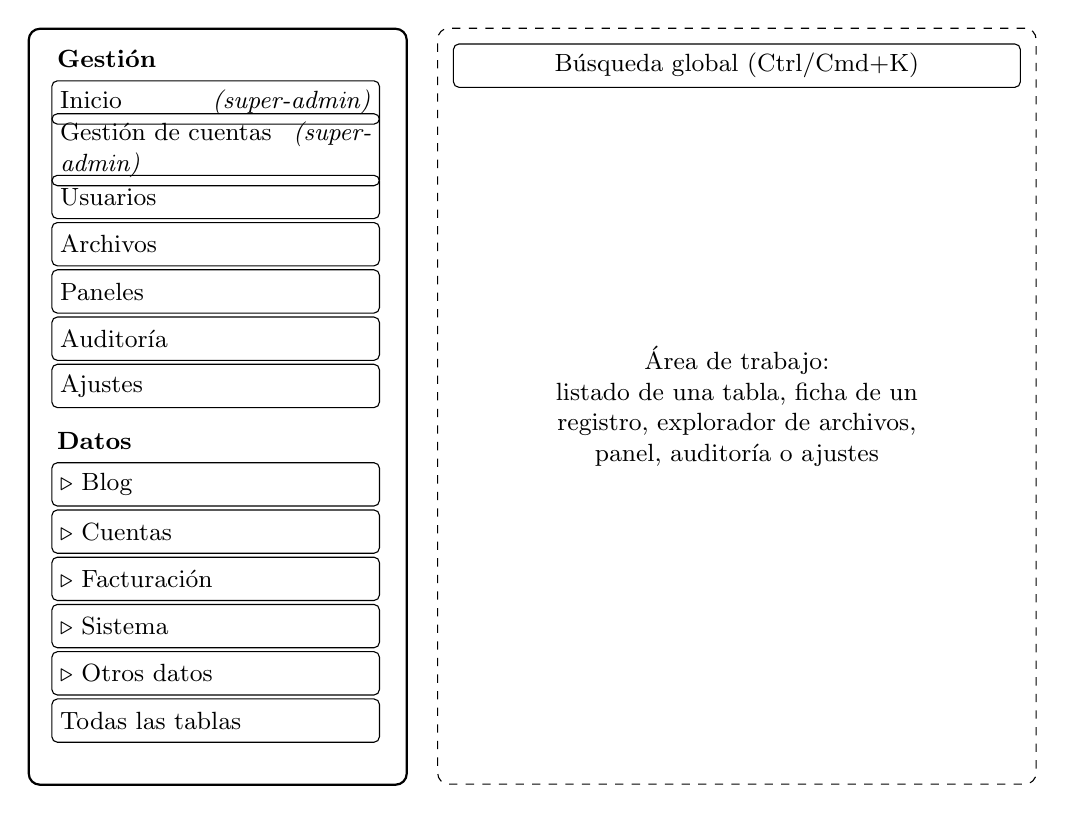
\begin{tikzpicture}[
      font=\small,
      box/.style={draw, rounded corners=2pt, text width=3.95cm, minimum height=0.55cm, anchor=west, inner sep=3pt},
      head/.style={font=\small\bfseries, anchor=west},
    ]
    \node[draw, thick, rounded corners=4pt, minimum width=4.8cm, minimum height=9.6cm, anchor=north west] (frame) at (0,0) {};
    \node[head] at (0.25,-0.4) {Gestión};
    \node[box] at (0.3,-0.95) {Inicio \hfill\textit{(super-admin)}};
    \node[box] at (0.3,-1.55) {Gestión de cuentas \hfill\textit{(super-admin)}};
    \node[box] at (0.3,-2.15) {Usuarios};
    \node[box] at (0.3,-2.75) {Archivos};
    \node[box] at (0.3,-3.35) {Paneles};
    \node[box] at (0.3,-3.95) {Auditoría};
    \node[box] at (0.3,-4.55) {Ajustes};
    \node[head] at (0.25,-5.25) {Datos};
    \node[box] at (0.3,-5.8) {$\triangleright$ Blog};
    \node[box] at (0.3,-6.4) {$\triangleright$ Cuentas};
    \node[box] at (0.3,-7.0) {$\triangleright$ Facturación};
    \node[box] at (0.3,-7.6) {$\triangleright$ Sistema};
    \node[box] at (0.3,-8.2) {$\triangleright$ Otros datos};
    \node[box] at (0.3,-8.8) {Todas las tablas};
    \node[draw, dashed, rounded corners=4pt, minimum width=7.6cm, minimum height=9.6cm, anchor=north west, align=center] (main) at (5.2,0) {};
    \node[align=center, text width=7cm] at (main.center) {Área de trabajo:\\ listado de una tabla, ficha de un\\ registro, explorador de archivos,\\ panel, auditoría o ajustes};
    \node[draw, rounded corners=2pt, anchor=north, minimum width=7.2cm] at ([yshift=-0.2cm]main.north) {Búsqueda global (Ctrl/Cmd+K)};
  \end{tikzpicture}
  \caption{Esquema de la consola de administración: bloques Gestión y Datos.}
  \label{fig:ug-consola}
\end{figure}

\subsection{Explorador de datos}
\label{sec:ug-datos}

Al elegir una tabla en el bloque «Datos» se abre su \textbf{listado}. Las
tablas y columnas aparecen con un nombre en español y, junto a él, su nombre
técnico. Desde el listado se puede:

\begin{itemize}
  \item paginar, ordenar por cualquier columna y buscar por texto;
  \item filtrar por columnas, con filtros adaptados al tipo de dato (fechas
        relativas como «últimos 7 días», valores de una lista o registros
        relacionados con autocompletado);
  \item elegir qué columnas se ven, fijarlas y reordenarlas, y guardar la
        combinación de filtros y columnas como una \textbf{vista guardada}
        para reutilizarla;
  \item seleccionar varios registros y eliminarlos en bloque, o editar un
        valor directamente en la celda (edición en línea).
\end{itemize}

Al pulsar un registro se abre su \textbf{ficha}, que muestra sus campos
agrupados según el diseño configurado y, debajo, los «Registros
relacionados» (por ejemplo, los miembros de una cuenta). Desde la ficha se
puede editar o eliminar el registro, crear un registro relacionado o vincular
y desvincular registros existentes. Para crear un registro nuevo se usa el
botón de alta del listado; el formulario valida los datos antes de guardarlos
y avisa si se intenta salir con cambios sin guardar.

\paragraph{Ejemplo: publicar una entrada del blog.}
Abra «Blog» $\rightarrow$ «Entradas», cree un registro nuevo, rellene el
título, el identificador para la dirección (\textit{slug}), el resumen, el
contenido en Markdown, la categoría, la imagen de portada y el estado de
publicación, y guárdelo. La entrada
aparecerá en \texttt{/blog} en cuanto esté publicada.

Todas las altas, modificaciones y bajas hechas desde la consola quedan
registradas en la auditoría con su autor, la fecha y los valores anteriores y
nuevos.

\subsection{Usuarios}
\label{sec:ug-usuarios}

«Usuarios» lista las personas registradas en la plataforma, con búsqueda y
filtros. La ficha de un usuario muestra sus datos y sus factores de
autenticación. Según los permisos, se puede crear o invitar a un
usuario, bloquearlo o desbloquearlo, enviarle un correo para restablecer la
contraseña o un enlace de inicio de sesión, quitarle un factor de dos pasos,
eliminarlo y conceder o revocar su acceso al CMS. Las acciones también pueden
aplicarse a varios usuarios a la vez. Cada acción pide confirmación.

\subsection{Archivos}
\label{sec:ug-archivos}

«Archivos» permite navegar por los contenedores de almacenamiento
(\textit{buckets}) y sus carpetas, subir archivos («Subir archivos»), crear
carpetas («Nueva carpeta»), renombrar y eliminar archivos y ver una vista
previa de los que la admiten, como imágenes y documentos PDF.

\subsection{Paneles}
\label{sec:ug-paneles}

«Paneles» reúne los paneles propios y los que otros han compartido con
usted. Un panel es una cuadrícula de \textit{widgets} de tres tipos: métrica
(un número, como las suscripciones activas), gráfica y tabla. Para crearlo,
pulse «Nuevo panel», añada \textit{widgets} con «Añadir widget» eligiendo la
tabla, los filtros y el tipo de representación, y colóquelos en la cuadrícula.
Un panel se puede renombrar, compartir con otros roles y eliminar. Cada
\textit{widget} muestra solo los datos que puede leer quien lo está viendo.

\subsection{Auditoría}
\label{sec:ug-auditoria}

«Auditoría» muestra los «Registros de auditoría»: quién hizo cada cambio,
cuándo, sobre qué tabla y registro, y cómo quedaron los datos antes y después.
Se puede filtrar por fecha, autor («Realizado por»), operación, tabla y
gravedad, y abrir el detalle de
una entrada para ver las diferencias. Las entradas las escribe el sistema y
nadie puede modificarlas; los datos que su rol no puede leer aparecen
ocultos.

\section{Super-administrador}
\label{sec:ug-superadmin}

El super-administrador es la cuenta raíz de la plataforma y del CMS: tiene
todos los permisos sin necesidad de configurarlos. Además de las herramientas
anteriores, dispone de:

\subsection{Inicio y gestión de cuentas}

\begin{itemize}
  \item \textbf{Inicio} (\texttt{/admin}): métricas de la plataforma
        ---«Usuarios», «Cuentas de equipo», «Clientes de pago» y «Pruebas»---,
        con la advertencia de que son estimaciones.
  \item \textbf{Gestión de cuentas} (\texttt{/admin/accounts}): listado de
        todas las cuentas, personales y de equipo, con búsqueda («Buscar
        cuenta\ldots») y filtro por tipo. En la ficha de una cuenta se ven sus
        equipos, sus miembros y su suscripción, y se puede:
        \begin{itemize}
          \item «Suspender» o «Reactivar» al usuario;
          \item «Suplantar» al usuario para ver la aplicación como él y darle
                soporte;
          \item «Enviar enlace de restablecimiento de contraseña»;
          \item eliminar la cuenta personal o la de equipo; y
          \item «Crear usuario», con la opción de confirmar su correo
                automáticamente.
        \end{itemize}
        Las acciones delicadas piden escribir la palabra
        \texttt{CONFIRMAR}.
\end{itemize}

\subsection{Ajustes de la consola}
\label{sec:ug-ajustes}

«Ajustes» agrupa la configuración del CMS en varias pestañas:

\begin{itemize}
  \item \textbf{General}: preferencias de la consola, como la zona horaria.
  \item \textbf{Autenticación}: si la consola exige verificación en dos pasos
        a todo el personal. Está activado por defecto y solo la cuenta raíz,
        con la sesión verificada en dos pasos, puede desactivarlo, porque
        afecta a toda la consola.
  \item \textbf{Miembros}: el personal con acceso a la consola. Permite
        «Cambiar rol», activar o desactivar a un miembro y consultar su
        auditoría. Nadie puede cambiar sus propios roles ni asignar un rol de
        rango superior al suyo.
  \item \textbf{Roles y permisos}: roles del CMS (por ejemplo, «Soporte»),
        grupos de permisos y permisos individuales sobre tablas,
        almacenamiento y herramientas. Un permiso puede conceder o denegar
        explícitamente una acción.
  \item \textbf{Recursos}: la configuración de cada tabla en la consola.
        \begin{itemize}
          \item «Sincronizar tablas» registra en el CMS las tablas nuevas de la
                base de datos.
          \item Para cada tabla se puede fijar su nombre visible y su
                descripción, su \textbf{área} en la barra lateral (por ejemplo,
                «Blog», o un área nueva para las tablas propias de la pyme),
                si es visible y su orden.
          \item Para cada columna, su nombre, su descripción ---que se muestra
                como ayuda «?» en los formularios---, si es visible o editable y
                su formato de visualización.
          \item «Registros relacionados» decide qué relaciones se muestran en
                la ficha, y «Diseño del registro» permite organizar los campos
                de la ficha en secciones arrastrándolos.
        \end{itemize}
\end{itemize}

\paragraph{Ejemplo: dar acceso limitado a una persona de soporte.}
\begin{enumerate}
  \item En «Usuarios», abra la ficha de la persona y elija «Conceder acceso al
        CMS».
  \item En «Ajustes» $\rightarrow$ «Miembros», asígnele el rol «Soporte» (o
        cree antes un rol a medida en «Roles y permisos» con los permisos de
        lectura de las tablas que necesite).
  \item Pídale que configure su segundo factor. Al entrar en la consola solo
        verá las áreas, tablas y herramientas que su rol le permite.
\end{enumerate}
